\section{}
\[
H(s)=\frac{100}{s^2+s+100}\,.
\]
\subsection{Bode-Diagramm}
\begin{center}
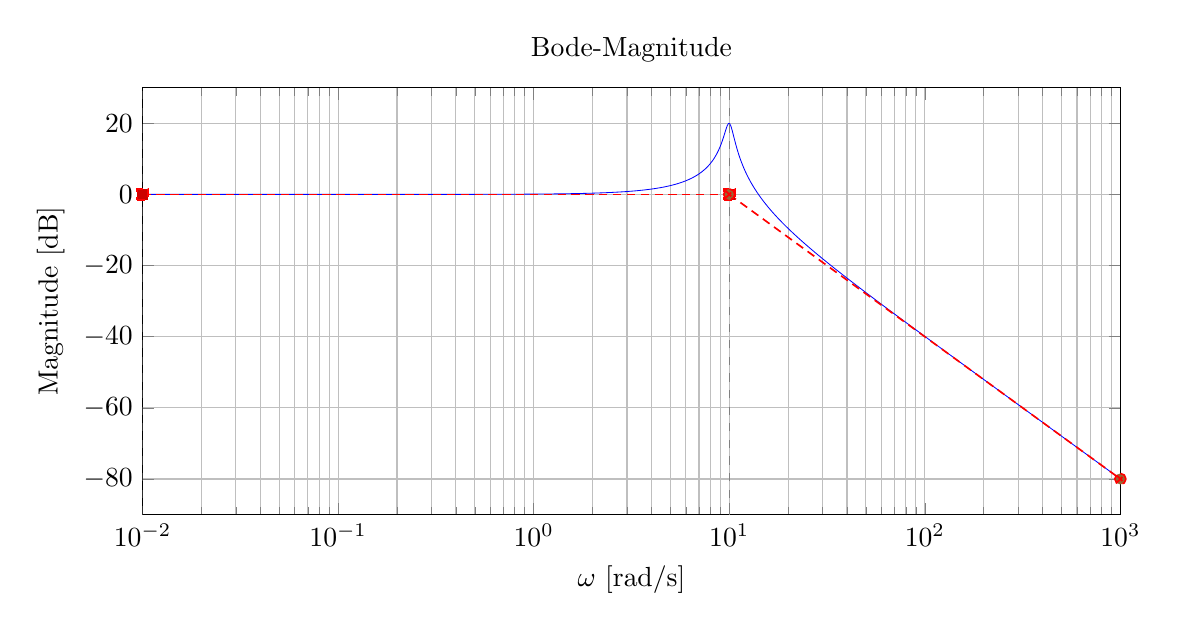
\begin{tikzpicture}
\begin{semilogxaxis}[
  width=14cm,height=7cm,
  xmin=1e-2,xmax=1e3,
  xlabel={$\omega$ [rad/s]},
  ylabel={Magnitude [dB]},
  ytick distance=20,
  grid=both,
  title={Bode-Magnitude}
]
\addplot[
  domain=1e-2:1e3,
  samples=800,
  mark=none,
  line width=0.3pt,
  blue
] {-10*ln((1 - (x/10)^2)^2 + (x/100)^2)/ln(10)};
\addplot+[domain=1e-2:1e1,samples=2,dashed,dash pattern=on 3pt off 2pt,line width=0.6pt,red] {0};
\addplot+[domain=1e1:1e3,samples=2,dashed,dash pattern=on 3pt off 2pt,line width=0.6pt,red] {-40*ln(x/10)/ln(10)};
\draw[gray,dashed] (rel axis cs:0,0) -- (rel axis cs:0,1);
\draw[gray,dashed] (axis cs:10,\pgfkeysvalueof{/pgfplots/ymin}) -- (axis cs:10,\pgfkeysvalueof{/pgfplots/ymax});
\node[gray,anchor=south east] at (axis cs:10,\pgfkeysvalueof{/pgfplots/ymax}) {\scriptsize Polpaar $\omega_n=10$, $\zeta=0.05$};
\end{semilogxaxis}
\end{tikzpicture}
\vspace{6mm}
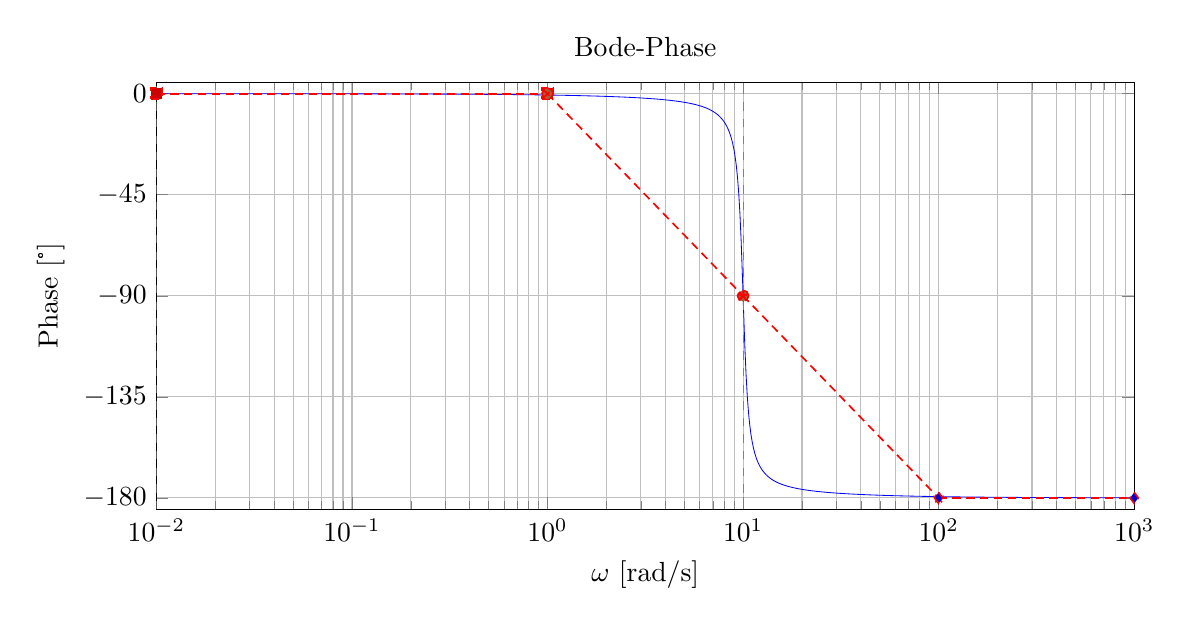
\begin{tikzpicture}
\begin{semilogxaxis}[
  width=14cm,height=7cm,
  xmin=1e-2,xmax=1e3,
  ymin=-185,ymax=5,
  ytick distance=45,
  xlabel={$\omega$ [rad/s]},
  ylabel={Phase [°]},
  grid=both,
  title={Bode-Phase}
]
\addplot[
  domain=1e-2:1e3,
  samples=800,
  mark=none,
  line width=0.3pt,
  blue
] {-atan2(x/100, 1 - (x/10)^2)};
\addplot+[domain=1e-2:1e0,samples=2,dashed,dash pattern=on 3pt off 2pt,line width=0.6pt,red] {0};
\addplot+[domain=1e0:1e1,samples=2,dashed,dash pattern=on 3pt off 2pt,line width=0.6pt,red] {-90*ln(x)/ln(10)};
\addplot+[domain=1e1:1e2,samples=2,dashed,dash pattern=on 3pt off 2pt,line width=0.6pt,red] {-90 - 90*ln(x/10)/ln(10)};
\addplot+[domain=1e2:1e3,samples=2,dashed,dash pattern=on 3pt off 2pt,line width=0.6pt,red] {-180};
\draw[gray,dashed] (rel axis cs:0,0) -- (rel axis cs:0,1);
\draw[gray,dashed] (axis cs:10,\pgfkeysvalueof{/pgfplots/ymin}) -- (axis cs:10,\pgfkeysvalueof{/pgfplots/ymax});
\node[gray,anchor=south east] at (axis cs:10,\pgfkeysvalueof{/pgfplots/ymax}) {\scriptsize Polpaar $\omega_n=10$, $\zeta=0.05$};
\end{semilogxaxis}
\end{tikzpicture}
\end{center}
\newpage
\subsection{Erklärung}
\vspace{5mm}
\begin{description}[leftmargin=1.2em,labelsep=.6em,font=\bfseries]
\item[Schritt 1] Normform: $s^2+s+100=\omega_n^2\!\left[\left(\tfrac{s}{\omega_n}\right)^2+2\zeta\left(\tfrac{s}{\omega_n}\right)+1\right]$ mit $\omega_n=10$ und $\zeta=\tfrac{1}{2\omega_n}=0.05$. DC-Faktor $100/100=1\Rightarrow 0\,\mathrm{dB}$ ohne Anfangssteigung; Startphase $\approx0^\circ$.
\item[Schritt 2] Konjugiertes Polpaar: Resonanz bei $\omega_n=10$. Asymptote $0\,\mathrm{dB}$ für $\omega\ll10$, ab $\omega=10$ Slope $-40\,\mathrm{dB/dec}$. Exakt liegt die Verstärkung bei Resonanz bei $|H(\j\omega_n)|=\tfrac{1}{2\zeta}=10\Rightarrow20\,\mathrm{dB}$.
\item[Schritt 3] Phase: Gesamtabfall\footnote{Im exakten Verlauf kippt die Phase schneller als von der Geradennäherung prognostiziert; Ursache ist das sehr kleine \(\zeta\). Je kleiner \(\zeta\), desto abrupter der Phasenübergang und desto schmaler sowie ausgeprägter die Resonanz im Magnitudenplot. Die handschriftliche Bode-Näherung ist hier grob; die genaue Lage der roten Segmente bleibt eine Abschätzung.} um $180^\circ$ um $\omega_n$, für die Geradennäherung über zwei Dekaden verteilt ($[1,100]$): $0^\circ\to-90^\circ$ in $[1,10]$, weiter $-90^\circ\to-180^\circ$ in $[10,100]$. Für $\omega\gg10$ nähert sich $\angle H\to-180^\circ$.
\end{description}

\vspace{0.5cm}
\medskip
\noindent\textbf{Stückweise Näherung}
\[
|H(\j\omega)|_{\mathrm{dB}}\approx
\begin{cases}
0,& \omega\ll10,\\[4pt]
+20,& \omega=10,\\[4pt]
-40\log_{10}(\omega/10),& \omega\gg10,
\end{cases}
\qquad
\]
\newpage